Quantum Chromodynamics (QCD) is a non-abelian gauge theory that describes the interactions between gluons and quarks. One of its central characteristics is the running of gauge coupling. At high energy scales, at which we have high-momentum transfer, the gauge coupling becomes very small resulting in gluons and quarks being almost free. This gives rise to the name asymptotic freedom. On the other hand we have a strong coupling for low-energy phenomena, in which the gluons and quarks cannot appear on their own, but only confined in hadrons\cite{bellac}. \\
The phase diagram of QCD is complicated and not fully understood. A sketch can be seen in figure \ref{fig:phase}. In very hot settings, for example at hundreds of MeV (trillions of Kelvin), hadron matter becomes deconfined and changes into the Quark-Gluon plasma (QGP). This state of matter occurs under extreme conditions such as in the core of heavy neutron stars and in ultra-relativistic heavy-ion collisions, which can be experimentally recreated in particle accelerators such as the LHC in CERN and RHIC in BNL\cite{phasediagram}. While understanding these phenomena is important on its own, it can also help to understand the early universe. Roughly $10^{-5}$\,s after the Big Bang matter was also a QGP\cite{monnai}.\\
\begin{figure}[H]
    \centering
    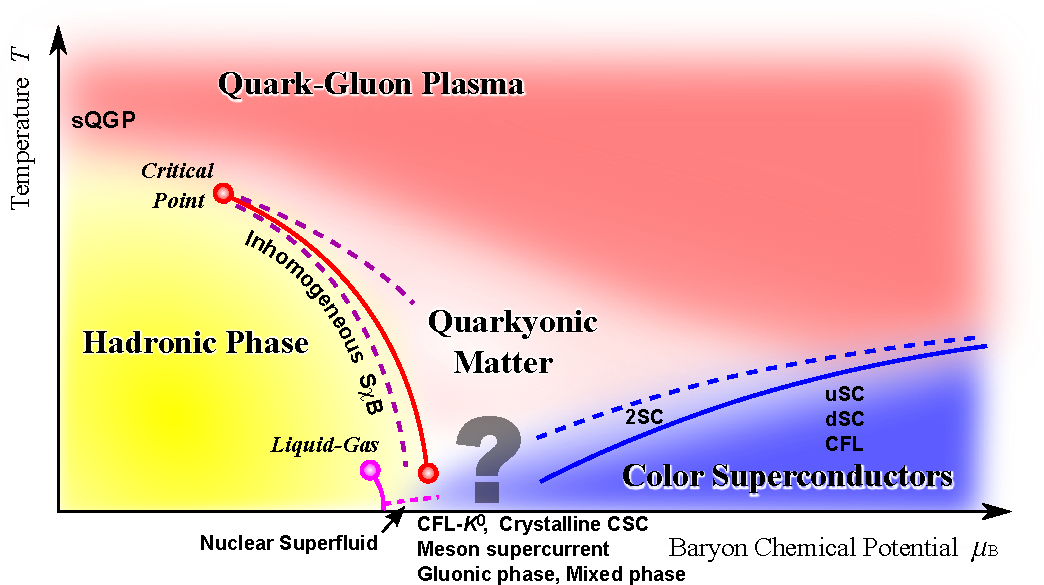
\includegraphics[width=0.7\linewidth]{images/phase.pdf}
    \caption{QCD Phase diagram \cite{phasediagram}}
    \label{fig:phase}
\end{figure}
Understanding these processes requires the equation of state, which is the reason for our calculation of the pressure in this thesis. To describe the theory in a more general setting, we would have to include the baryon chemical potential. However, this would make the calculation even more complicated, since its inclusion would invoke the sign problem which would make a direct lattice calculation impossible. Pavan et al. \cite{pavan} was able to compute the pressure for non-vanishing chemical potential. The uncertainties of their results are dominated by uncertainties of the literature values for the pressure for vanishing chemical potential. We hope to reduce these errors by providing a high precision measurement of the pressure for vanishing chemical potential.\\
A high-precision pressure measurement would also be useful and needed for the renormalization of the Energy-Momentum-Stress Tensor (EMT). The EMT can then be used to describe the hydrodynamics of the QGP. 


